\documentclass[9pt]{beamer}
\usepackage{kotex}
\usepackage{amsfonts,amssymb,amsthm}
\usepackage[dvipsnames]{xcolor}
\usepackage{xcolor}
\usepackage{etoolbox}
\usepackage{braket}
%## color
\definecolor{customBlack}{HTML}{3B4252}
\definecolor{customBlackGrey}{HTML}{434C5e}
\definecolor{cuatomGrey}{HTML}{4C566A} 
\definecolor{customWhite}{HTML}{ECEFF4} 
\definecolor{customBlue}{HTML}{6082B6}  
\definecolor{customRed}{HTML}{BF616A}
\definecolor{vividauburn}{rgb}{0.58, 0.15, 0.14}


%## Theme & custom
% \usetheme{metropolis}           % Use metropolis theme
% \metroset{block=fill}
\usetheme{moloch} % modern fork of the metropolis theme
\molochset{block=fill}
\setbeamersize{text margin left=5mm, text margin right=5mm}
\setbeamercolor{palette primary}{bg=customBlack}
\setbeamercolor{alerted text}{fg=customRed}
\setbeamercolor{itemize item}{fg=customBlue}
\setbeamercolor{enumerate item}{fg=customBlue}


%## font
\usefonttheme[onlymath]{serif}
% \setbeamerfont{normal text}{size=\small}
% \setbeamerfont{math text}{size=\tiny}


%## Theorem title, numbering
\makeatletter
\setbeamertemplate{theorem begin}
{%
\begin{\inserttheoremblockenv}
{%
\inserttheoremheadfont
\inserttheoremname
\ifx\inserttheoremaddition\@empty\else\ of\ \inserttheoremaddition\fi%
\inserttheorempunctuation
}%
}
\setbeamertemplate{theorem end}{\end{\inserttheoremblockenv}}
\makeatother
\setbeamertemplate{theorems}[numbered]  


%## Custom block
\setbeamercolor{block title}{bg=customBlue, fg=white}
\setbeamercolor{block body}{bg=customWhite, fg=customBlack}
\setbeamercolor{block title alerted}{%
    use={block title, alerted text},
    bg=customRed,
    fg=white
}
\setbeamercolor{block body alerted}{%
    use={block title, alerted text},
    bg=customWhite,
    fg=customBlack
}
\AtBeginEnvironment{definition}{%
    \setbeamercolor{block title}{fg=white,bg=customBlackGrey}
    \setbeamercolor{block body}{fg=customBlack, bg=customWhite}
}
\AtBeginEnvironment{theorem}{%
    \setbeamercolor{block title}{fg=white,bg=customBlackGrey}
    \setbeamercolor{block body}{fg=customBlack, bg=customWhite}
}
\AtBeginEnvironment{corollary}{%
    \setbeamercolor{block title}{fg=white,bg=customBlackGrey}
    \setbeamercolor{block body}{fg=customBlack, bg=customWhite}
}
\AtBeginEnvironment{lemma}{%
    \setbeamercolor{block title}{fg=white,bg=customBlackGrey}
    \setbeamercolor{block body}{fg=customBlack, bg=customWhite}
}


%! Useful command
\renewcommand{\Pr}{\text{Pr}}
% $\ast$ \underline{Proof}:
%\checkmark \underline{meaning}:

\title{3. Basics of Classical Computer}
\date{\today}
\author{Vaughan Sohn}
% \institute{Centre for Modern Beamer Themes}


\begin{document}
    %#################################### 
    \maketitle
    
    %#################################### 
    \begin{frame}
        \frametitle{Contents}
        \tableofcontents
    \end{frame}


    %#################################### 
    \begin{section}{Turing machine}
        \begin{frame}{Definition of Turing machine}
            \textbf{Components of a Turing machine}
            \begin{itemize}
                \item State: TM이 가질 수 있는 state들의 finite set $\{Q\}$
                \item Transition function: TM이 tape에서 symbol을 읽고 자신의 state에 따라서 어떻게 동작할 것인지를 결정하는 \textit{partial} function.
                $$ \delta : Q \times S \rightarrow Q \times S \times \{L, N, R\}$$
                \item Tape: input string이 적인 infinite length의 메모리.
                \begin{itemize}
                    \item $S$: tape에 쓰일 수 있는 모든 symbol들의 finite set $\{blank, \#, \ast\} \subseteq A$
                    \item $A$: $S$의 부분집합 $\{blank, \#\} \nsubseteq A$
                \end{itemize}
                \item Read/Write Head: tape에서 symbol을 읽고 쓰는 위치를 나타내는 head.
            \end{itemize}
            \begin{figure}
                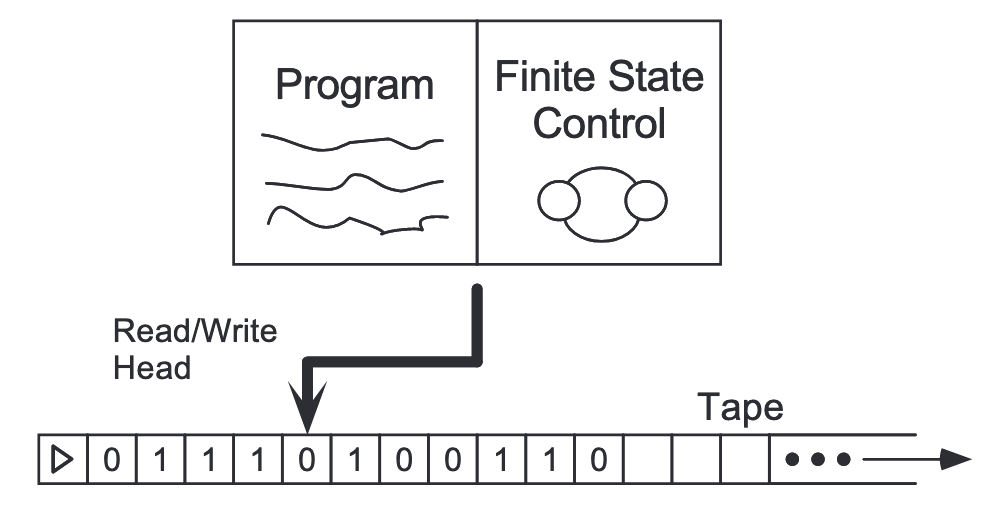
\includegraphics[width=0.5\columnwidth]{image/L3_turing_machine.png}
            \end{figure}
        \end{frame}

        \begin{frame}{Definition of Turing machine}
            \textbf{Operation of a Turing Machine}
            \\turing machine $M$, 그리고 input string $x$에 대하여,
            \begin{enumerate}
                \item initial state $q_0$으로 초기화한다.
                \item input string $x$를 tape에 작성한다. (남은 부분은 blank)
                \item halt가 되지 않으면, 매 step마다 다음을 반복한다.
                \begin{enumerate}
                    \item head위치 $i$에서 symbol $s_i$를 읽는다.
                    \item transition function을 참고하여 $(q, s_i)$일 때, 어떻게 행동해야하는지를 구한다.
                    \item transition function의 규칙에 따라 symbol, state, head를 업데이트한다. \\ $ \Rightarrow (q', s_i', i+\Delta h)$
                \end{enumerate}
            \end{enumerate}

            \vspace{0.8cm}
            \textit{Halting 규칙은 다음과 같다.}
            \begin{itemize}
                \item head가 tape의 범위를 벗어났을 때
                \item $(q, s_i)$에 대한 transition function이 정의되지 않았을 때
                \item $s_i = \#$일 때
            \end{itemize}
        \end{frame}

        \begin{frame}{Universial Turing machine}
            \begin{definition}
                A machine that can solve any problem is called a \textbf{Universial Turing machine}.
            \end{definition}
            \begin{itemize}
                \item UTM은 자신이 시뮬레이션 할 TM의 index $i$와 그 TM의 시뮬레이션에 사용할 input$x$을 입력으로 받게 된다. ($i$, $x$)
                \item UTM의 program; transition function안에는 각각의 TM에 대한 동작이 모두 기술되어있기 때문에 그 내용을 따라서 진행하면 $M_i(x)$의 결과를 얻게되고, 이를 output으로 반환하게된다.
                $$ U(i, x) = \varphi_{M_i}(x)$$
                \item 각 Turing machine의 state, symbol은 모두 \alert{finite set}이며, 따라서 transition function도 finite하기 때문에 모든 TM에 대한 내용을 하나의 TM $U$에 담을 수 있다.
            \end{itemize}
        \end{frame}

        \begin{frame}{Church-Turing thesis}
            \begin{definition}
                A partial function $f: A^* \rightarrow A$ is computable if there exists a Turing machine $M$ such that $\varphi_M = f$. In this case, we say that $f$ is computed by $M$.
            \end{definition}
            \begin{block}{Church-Turing thesis}
                The class of functions computable by a Turing machine corresponds exactly to the class of functions which we would naturally regard as being computable by an algorithm.
            \end{block}
            \begin{itemize}
                \item Church-Turing thesis는 실제 알고리즘과 튜링머신을 연관시켜 생각하는 강력한 가설이다.
                \item 그러나, TM이 모든 function을 계산할 수 있는 것은 아니다! (e.g., Halting problem)
            \end{itemize}
        \end{frame}
        
        \begin{frame}{Halting problem}
            \begin{alertblock}{Halting problem}
                Dose turing machine $M$ halt for given input $x$?
                \\ $\rightarrow$ \textit{We can't compute halting problem by any turing machine!}
            \end{alertblock}
            \vspace{0.2cm}
            $\ast$ \underline{Proof}:
            (귀류법) Halting 문제를 풀 수 있는 TM $\text{HALT}$가 존재한다고 가정하자.
            \vspace{5cm}

        \end{frame}

    \end{section}


    \begin{section}{Circuit model}
        \begin{frame}{Definition of Circuit model}
            \textbf{Circuit model}
            \begin{columns}
                \begin{column}{0.6\textwidth}
                    \begin{itemize}
                        \item 무한히 긴 메모리(tape)를 가지는 이상적인 TM 대신, circuit model을 사용할 수도 있다.
                        \item Circuit; 회로는 wire와 gate로 이루어진다.
                        \begin{itemize}
                            \item wire: bit value가 전달되는 길
                            \item gate: 각 single/multi bit에 대해 연산을 수행하는 장치
                        \end{itemize}
                        \item 각 gate는 오른쪽과 같은 symbol로 표현된다.
                    \end{itemize}
                \end{column}
                \begin{column}{0.45\textwidth}  %%<--- here
                    \begin{center}
                        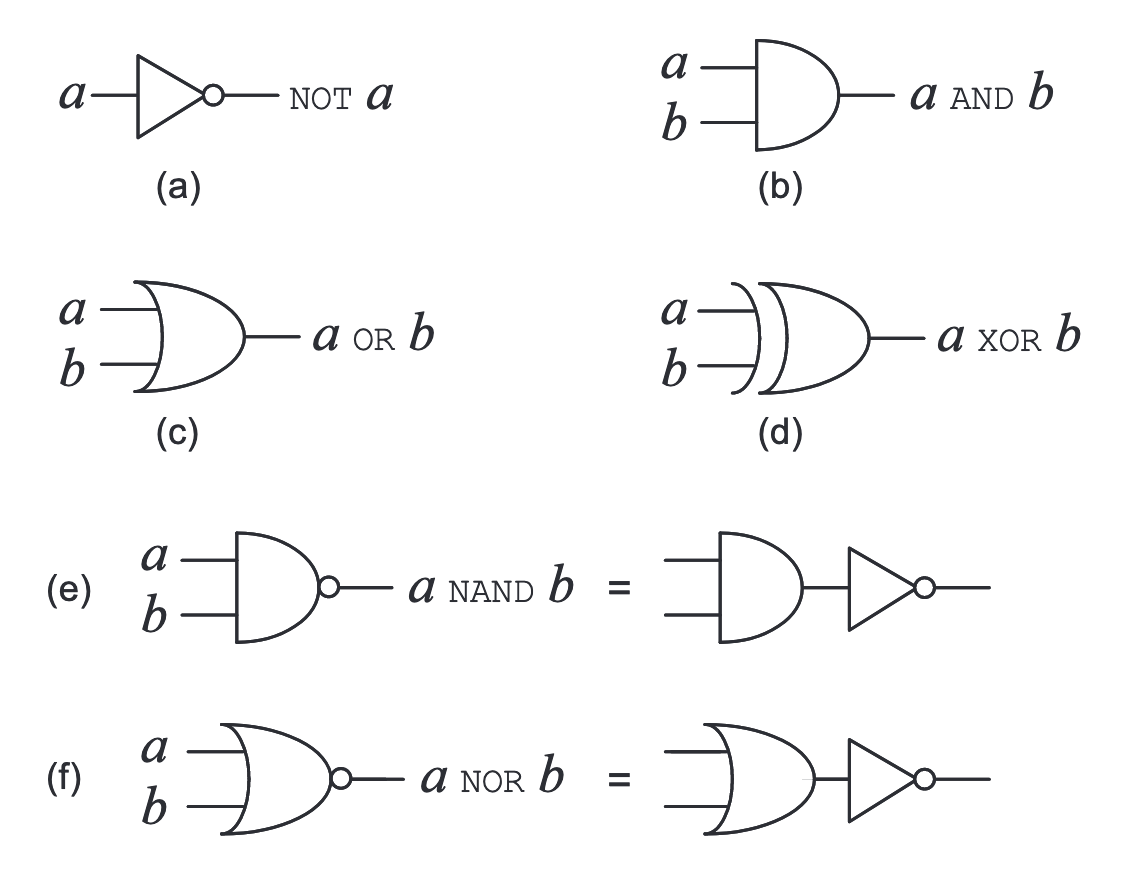
\includegraphics[width=0.95\columnwidth]{image/L3_gate_symbol.png}
                    \end{center}
                \end{column}
                \end{columns}
        \end{frame}

        \begin{frame}{Universiality of Circuit model}
            \begin{theorem}
                Circuit model can solve every type of boolean function.
                $$f : \{0, 1\}^n \rightarrow \{0, 1\}^m$$
            \end{theorem}
            \vspace{0.2cm}
            $\ast$ \underline{Proof}: (mathematical induction)
            \begin{itemize}
                \item 먼저 $n=m=1$인 boolean function에 대해 생각해보자. 이 함수는 앞에서 언급한 gate들을 이용하여 쉽게 구현할 수 있다.
                \item (귀납적 가정) $m=1$일 때, 어떤 $n$에 대해서도 boolean function을 구현할 수 있는 회로가 존재한다고 가정하자.
                \item 그럼 $n+1$에 대한 boolean function은 $n+1$번쨰 bit값이 0인지 1인지에 따라서 동작하는 서로다른 $n$bit function $f_0, f_1$을 사용하여 구현할 수 있다.$\Box$
            \end{itemize}
        \end{frame}
    \end{section}

        \begin{frame}{Computation power of Circuit model}
            % TM은 infinite한 크기의 tape를 가지지만, circuit model은 정해진 input bit를 가지며, 만약 더 긴 input에 대해 회로를 구성하기 위해서는 다른 설계를 해야한다.
            \begin{alertblock}{Can circuit model solve halting problem?}
                Circuit model은 어떤 boolean function도 구현할 수 있기 때문에, \textit{halting problem을 푸는 function}도 구현할 수 있다! 그러나 halting problem을 푸는 회로 $h_n$을 어떻게 설계해야하는지 알 수 없기 때문에 여전히 halting problem은 풀 수 없다.
                \\ \textit{$\Rightarrow h_n$ is \alert{non-uniform circuit family.}}
            \end{alertblock}
            \begin{definition}[circuit and circuit family]
                A \textbf{circuit family} consists of a collection of circuits, $\{C_n\}$. The circuit $C_n$ has $n$ input bits and the output of the circuit $C_n$, upon input $x$ ($len(x) \le n$) is denoted by $C_n(x)$.
                The function computed by the circuit family $\{C_n\}$ is the function $C(·)$.
            \end{definition}
            \begin{itemize}
                \item uniform circuit family: $C(\cdot)$에 대해, 어떠한 입력 크기 $n$에 대해서도 회로 $C_n$의 구조를 출력하는 알고리즘이 존재하는 회로 집합.
                \item non-uniform circuit family: $C(\cdot)$에 대해, 어떠한 입력 크기 $n$에 대해서도 회로 $C_n$의 구조를 출력하는 알고리즘이 존재하지 않는 회로 집합.
            \end{itemize}
        \end{frame}


    %#################################### 
    \begin{frame}{References}
        
        \begin{itemize}
            \item M. A. Nielson and I. L. Chuang, Quantum Computation and Quantum Information
            \item Lecture notes for QU511: Quantum Computing (Fall 2024)
        \end{itemize}
        \vspace{6cm}
    \end{frame}

\end{document}